\documentclass[11pt,
  titlepage=false,
  %parskip=half,      % enable if you want paragraphs separated by vertical spacing instead of indents
]{scrreprt}

% Style settings
\usepackage[utf8]{inputenc}
\usepackage{microtype}
\usepackage[T1]{fontenc}
\usepackage{lmodern}
\addtokomafont{disposition}{\rmfamily}

% Hack chapter layout - don't use in other papers!
\usepackage{etoolbox}
\makeatletter\patchcmd{\scr@startchapter}{\if@openright\cleardoublepage\else\clearpage\fi}{}{}{}\makeatother

% Useful packages for complex content:
\usepackage{amsmath,amsfonts,amssymb} % typesetting math
%\usepackage{siunitx}                 % typesetting SI-units and formatted numbers
%\usepackage{listings}                % typesetting source code
\usepackage{booktabs,multirow}        % utils for complex/beautiful tables
%\usepackage{subcaption}              % placing multiple subfigures in a figure
%\usepackage{graphicx}                % including external image files
%\usepackage{tikz}                    % drawing figures within LaTeX

% Bibliography, referencing, and indexing
\usepackage{csquotes}                 % typesetting \enquote{text in quotes} correctly
\usepackage[backend=biber,
            style=alphabetic,
            minalphanames=3, maxalphanames=4,
            maxbibnames=20]{biblatex} % to generate the bibliography
\addbibresource{report.bib}           % name of the bib-file

% Useful utils:
%\usepackage{todonotes}               % add ToDo markers (\todo{...}, \todo[inline]{...})
\usepackage[hidelinks]{hyperref}
\usepackage{textcomp}
\usepackage{graphicx}      % clickable links (but hide color frames around links)
%\usepackage{cleveref}                % named references (\Cref{chap:introduction}, ...)

% Your own macros:
%\newcommand{\mynewmacro}[1]{my content with one input parameter: #1}


\begin{document}

%--- FRONT MATTER --------------------------------------------------------------

\title{JavaSQUIP}
\subtitle{An application of a scheduler queue-based covert channel to JavaScript}
\author{Christoph Royer}
% TODO change to Backelor's thesis
\date{Introduction to Scientific Working 2022/23\bigskip\bigskip}
\publishers{\normalsize
  Supervisor:
  Stefan Gast
  \medskip\par
  Institute of Applied Information Processing and Communications\\
  Graz University of Technology
}


\maketitle

\chapter*{\centering\Large Abstract}
\label{ch:abstract}
The implementation of out-of-order execution has brought a big performance benefit to current CPUs.
But with this benefit also come security concerns, since attackers can exploit the timing variations which are bound to occur in an out-of-order pipeline.
Attacks which target only one execution unit through a separate scheduler queue -- as seen in the Apple M1 and AMD Zen 2 and Zen 3 microarchitectures -- have proven even more powerful than port contention on single-scheduler systems.
As with any attack, porting this side channel to the web would greatly increase its reach and number of victims.

In this paper, we present the JavaSQUIP attack, which is a port of SQUIP~\cite{squip} to JavaScript.
We look into the security measures used in common browsers to prevent timing attacks, and show how we worked around them successfully.
Our covert channel can provide communication across separate browser instances at a speed of 1000 bits/s, which is faster than any current covert channel of this type.
% TODO add eval data

JavaSQUIP makes it clear that current browsers have not yet been able to adapt to be secure in light of the ever increasing complexity of modern CPUs.
Our findings suggest that making these attacks impossible may not even be feasible because the drawbacks in performance and features would be too large.
\paragraph{Keywords:}
Covert channel $\cdot$
Scheduler queue contention $\cdot$
JavaScript $\cdot$
AMD Zen

\clearpage

%--- INTRODUCTION --------------------------------------------------------------

\chapter{Introduction}
\label{ch:introduction}

Nowadays, CPU manufacturers are in a steady competition against each other to make their product faster and faster.
One of the ways this is achieved is \textit{out-of-order execution}, where instructions are not executed in the order given by the binary,
but rather as soon as their respective dependencies are ready and a suitable execution unit is free.
Although this toes the line of breaking the hardware-software contract, the CPU ensures that out-of-order execution remains transparent to the user.
To better balance usage of its execution units, modern CPUs often also include \textit{Simultaneous Multithreading} (SMT).
Here, one physical core is split up into two logical cores, which share physical infrastructure like the schedulers and execution units.

Though out-of-order execution and SMT are designed to be transparent to the user, attacks like
SMoTherSpectre~\cite{Bhattacharyya2019} and PortSmash~\cite{Aldaya2019port} show that the combination of the two forms a viable attack surface.
By measuring timing variations in out-of-order execution, an attacker can gain insight into sensitive information.
The two attacks achieve this is through \textit{port contention}.
%Because the instructions are reordered on the fly, the CPUs scheduler needs to distribute incoming instructions across the ports for its several specialized execution units.
If the attacker is co-located with the victim on the same core, they can measure delays when issuing instructions to a shared execution unit.
In this way, the attacker can gain knowledge on the victim's execution based on whether instructions are delayed by the scheduler or not.

SQUIP~\cite{squip} focuses on CPUs with multiple specialized scheduler queues to implement \textit{scheduler queue contention}.
Because each scheduler deals with fewer execution units, the attacker can push one of the comparatively small scheduler queues close to its capacity.
If the victim also adds to the queue, the pipeline stalls, which results in a big spike in execution time
This makes SQUIP a fast and reliable covert channel on many modern CPU architectures such as the AMD Zen 2 and Zen 3.
% TODO add graphic

Since implementations of port contention-based side channels in a browser setting already exist~\cite{Rokicki2022webport}, we ask the following research question:

\textit{Can per-execution-unit scheduler queue contention be exploited in a browser setting? Are there significant benefits compared to single scheduler port contention-based approaches?}

In this paper, we present JavaSQUIP, a browser-based covert channel using the SQUIP attack.
We show that it is reliable and faster than approaches based on CPU architectures with a single scheduler queue.
We develop a framework for transmitting data between separate instances of a browser at speeds of up to 1000 bit/s.

% TODO Update outline
\paragraph{Outline.}
In Section~\ref{ch:background}, we provide relevant background information on pipelines, schedulers and scheduler queue contention.
We also observe several challenges that come with trying to implement a timing attack in a browser.
Section~\ref{ch:implementation} shows how we dealt with these challenges.
We go into more detail on the mode and results of our evaluation of JavaSQUIP in Section~\ref{ch:evaluation}.
Section~\ref{ch:conclusion} concludes by comparing JavaSQUIP's performance to similar attacks and outlining potential use cases.


%--- BACKGROUND ----------------------------------------------------------------

\chapter{Background}
\label{ch:background}

In this chapter, we go into detail on CPU scheduling and how it has been exploited in the past.
Afterwards, we take a closer look into the browser features needed to implement these exploits in JavaScript.

\section{CPU Scheduling}
\label{sec:cpuschedulers}
For performance reasons, modern CPUs use efficiency features at almost every stage of an instruction's execution.
In the following, we will list some of these features for each of the stages along with the way they are exploitable.

\textbf{Fetch.}
Before an instruction can be executed, it needs to be loaded from cache or memory.
As branches can make loading unpredictable and loading the wrong instruction is expensive, a \textit{branch prediction unit} tries to guess which path is more likely to be loaded.
Taking this one step further, the predicted path may also be executed before the condition for the branch has been computed.
This is called \textit{speculative execution}\cite{AMD2020OptimizationEPYC7002}, and it can be exploited, as was shown in the Spectre~\cite{spKocherHFGGHHLM019} attack.

% TODO add SMT clarification
\textbf{Decode.}
Modern CISC CPUs divide normal instructions into smaller instructions;
these are called \textit{micro-ops} (\textmu ops)\cite{AMD2020OptimizationEPYC7002}.
For example, an addition with memory operands may be split up into three \textmu ops: one for loading the operands, one for the addition, and one for storing the result.
These \textmu ops can be distributed across specialized execution units, enabling more parallelisation and load balancing, and thus an increase in performance.

% TODO elaborate scheduler queues
\textbf{Schedule/Execute.}
Once created, the \textmu ops are queued to be executed as soon as their dependencies are met -- sometimes out of the order of their arrival.
Depending on the CPU micoarchitecture, there can be one general scheduler queue for all execution units, or multiple.
On CPUs that support simultaneous multithreading (SMT), an attacker may be co-located with the victim on the same core.
This opens up two vectors for a timing attack: \textit{port contention} and \textit{scheduler queue contention}.

SMoTherSpectre~\cite{Bhattacharyya2019} and PortSmash~\cite{Aldaya2019port} implement port contention.
They use the fact that only one of the two threads in an SMT-enabled core can use an execution unit in a single cycle.
The attacker can thus find out whether the victim is using a port by measuring the execution time of an instruction on the same port.

SQUIP~\cite{squip} on the other hand implements scheduler queue contention.
In scheduler queue contention, the attacker fills up the scheduler queue to the point that it is almost at its capacity limit;
any activity of the victim that involves this scheduler queue will overflow the queue, leading to a queue stall.
The attacker can measure this easily because it entails a significant spike in execution time in the affected queue.
% TODO visualisation of sqc

\clearpage
SQUIP is limited in its applicable CPU architectures because it relies on the split-scheduler architecute of AMD Zen2 and Zen3 CPUs to distinguish between \textmu ops.
However its advantage is a higher transmission rate compared to port contention.
Because of this, JavaSQUIP aims to port this vulnerability to a browser environment.
% TODO Because of what?

% TODO add Zen3
\begin{figure}
    \centering
    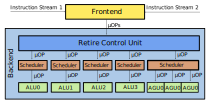
\includegraphics[width=0.5\textwidth]{figures/Zen2 arch}

    \caption{The scheduler layout in AMD Zen2 (c.f.~\cite{AMD2017OptimizationEPYC7001})}
    \label{fig:amdzen2}
\end{figure}

\textbf{Retire.}
After all the \textmu ops of an instruction have completed, the \textit{retire control unit} (RCU) reassembles the results.
It commits the finished instructions and schedules dependent instructions -- the dissection into \textmu ops is transparent to the user.


\section{Browser security measures}
\label{sec:browsersecurity}
Since the advent of many timing side- and covert channels~\cite{noack2018exploiting, Rokicki2022webport, gruss2016rowhammer},
browser developers have implemented many measures to mitigate the threat~\cite{shusterman2021prime, performancenow, performancenowchrome}.
This has always meant striking a balance between security and efficiency.
Because of this, many potential attack surfaces cannot be eliminated without unreasonable losses in performance and functionality,
though some measures do slow down side- and covert channels significantly.

In the following we expand on security measures regarding multithreading, accurate timing in browsers, and low-level operations.
All three of these are needed to mount the SQUIP attack.


\subsection{Timing functions}\label{subsec:timingjs}
There are two contenders for timing measurements in JavaScript: \texttt{Date.now()}~\cite{datenow} and \texttt{performance.now()}~\cite{performancenow}.

% TODO word repetition
The \texttt{Date.now()}~\cite{datenow} function gives a synchronized Unix epoch timestamp with millisecond accuracy.
This is synchronized across all contexts and browser instances.

% TODO timeorigin
\texttt{performance.now()} measures the time elapsed since the \textit{time origin} of the current context.
This means that \texttt{performance.now()} gives different values between browser instances, and even between a main thread and its worker threads.
The accuracy of \texttt{performance.now()} has been heavily restricted by browsers to counteract the threat of timing attacks.
For example, in Firefox it has an accuracy of 1 ms, and in Chrome it measures with an accuracy of 0.1 ms~\cite{performancenow, performancenowchrome}.

\subsection{Multithreading}\label{subsec:multithreading}
Though JavaScript does not support low-level control over threading, the \texttt{Web Workers} API~\cite{webworkers} allows the user to create workers running in a separate thread.
An instantiated worker runs a predefined script.
The main thread can interface with the worker via calls to the \texttt{Worker.postMessage()} function and via a \texttt{SharedArrayBuffer}~\cite{sharedarraybuffer}.
There is no support for selecting a core on which a worker is run on, presenting a challenge to co-locate with the sender.

Creating a \texttt{SharedArrayBuffer} was restricted in two ways: the browser window needs to be SSL-encrypted, and it needs to restrict some Cross-Origin requests.
Nevertheless, this is not a problem for this attack since the site provides \texttt{https} and all code comes from a single origin.


\subsection{Low-level operations in JavaScript}\label{subsec:lowleveljs}
JavaScript handles numbers as floats by default.
This means that a simple invocation of a multiplication like \texttt{a * b;} in JavaScript will not result in an \texttt{imul} instruction on the CPU.
Rather, \texttt{Math.imul(a, b)}~\cite{mathimul} gives the user a lower-level command:
It interprets the parameters as 32bit integers and multiplies them as such, resulting in an \texttt{imul} instruction on the CPU.


%--- IMPLEMENTATION ----------------------------------------------------------------
\chapter{Implementing JavaSQUIP}
\label{ch:implementation}
As described in Section~\ref{sec:browsersecurity}, there are some challenges to overcome when implementing a timing attack in a browser.
This chapter explains how we worked around these challenges to implement the JavaSQUIP covert channel.

\section{Getting accurate timing}
\label{sec:accurate-timing}
JavaSQUIP needs two kinds of timing in order to work properly:
\begin{itemize}
    \item a cross-browser syncronized clock to determine the start of bit transmissions:\\
    resolution of ${f_{\text{transmission}}}^{-1} \approx$ 1ms
    \item a fine-grained measurement to measure port contention:\\
    resolution of 100 CPU cycles $\approx$ 25ns
\end{itemize}

For the synchronized clock, we can use \texttt{Date.now()}~\cite{datenow}, which has a 1ms accuracy.
This method only works for transmissions of up to 1000 bits/s, since there is no more precise timestamp in JavaScript which is synchronized across browser instances.

%To get around this and realize a faster transmission than 1000 bits/s, we propose implementing the Manchester Code~\cite{manchesterEncoding}.
%It is self-synchronizing, which eliminates the need for an external source of synchronisation.
%The actual implementation is not within the scope of this paper.

The receiver also needs a way to measure the small variations in timing whenever a scheduler queue gets blocked.
Since no timing function in JavaScript gives a better accuracy than 0.1ms, we need to provide our own timing.

We solved this with a counting worker, which continually increases one variable in the \texttt{SharedArrayBuffer}.
As explained in section \ref{subsec:multithreading}, the other receiver workers can then access this counter and use it to measure execution times with adequate accuracy.

%TODO explain timeslices, start of bytes

\section{Co-locating with the sender}
\label{sec:co-location}
For co-locating the receiver with the sender, the receiver creates as many receiving workers as the number of virtual cores in the machine, minus two:
one for the counting thread (see \ref{sec:accurate-timing}), and one for the sending thread.
For the 8-core CPUs we used in our experiments (TODOCPU), this comes to $8 \times 2 - 2 = 14$ receiver workers.
Since every thread does continuous work, each thread will most likely be assigned to a unique virtual core.

To receive the message, one of the worker threads needs to be co-located with the sending thread.
Assuming a uniform distribution for the threads, we can calculate the theoretical co-location probability.
The only way that the sender is not co-located with a receiver is that the sender is co-located with the counting thread,
which is a $\frac{1}{15}$ chance.
Thus, the theoretical co-location probability is $\frac{14}{15} \approx 93.3\%$

% TODO link to graphics
\section{Targeting a scheduler queue}
JavaSQUIP targets AMD Zen, Zen2, and Zen3;
these architectures support multiplication only on ALU1~\cite{AMD2020OptimizationEPYC7003}.
JavaSQUIP fills up the scheduler queue of ALU1 by making multiple codependent calls to \texttt{Math.imul()}, which translate to the \texttt{imul} instruction.


%--- EVALUATING JAVASQUIP --------------------------------------------------------------
\chapter{Evaluating JavaSQUIP}
\label{ch:evaluation}

To evaluate and measure different approaches, we set up a test scenario for JavaSQUIP.
It consists of two web pages communicating with each other solely over JavaSQUIP.

\section {Test setup}
\label{sec:testsetup}
The test setup is comprised of two webpages: a sender and a receiver.
The sender simulates the target, and the receiver simulates a page that is controlled by the attacker.
Because the attacker has little or no control over the target, we kept the sender page minimal.
The sender has only one working thread.
The working thread is sending either a 0 (no action) or a 1 (contention with codependent \texttt{Math.imul()} calls) for each timeslice.
With more control over the receiver, the attacker can ensure co-location from this side.
For our tests on \textbf{TODOCPU1} (Zen2) and \textbf{TODOCPU2} (Zen3), we needed 14 receiving workers.
We go into more detail on co-location in Chapter~\ref{sec:co-location}.

To distinguish a message from random noise on the CPU, the sender sends a preamble before the actual data.
The preamble is a sequence of the numbers from 100 through 109.
If the receiver sees two ascending bytes between 100 and 109, it is highly likely that this is part of the preamble --
a message was detected.
For easier evaluation of the transmission accuracy, the message is also stored on the receiver's side,
so that the number of "faulty 1" and "faulty 0" bits can be automatically calculated.
In our test setup, messages of 500 random bytes were sent at a transmission speed of 1000bits/s.
This results in a transmission time of $\frac{500 \dot 8}{1000} = 4$ seconds.

\section{Speed}
The sender and receiver need to know the desired transmission speed beforehand to match up their timeslices.
This means that the transmission speed is a fixed value and needs no further calculation.
Due to reasons explained in Section~\ref{sec:accurate-timing}, our best acheivable speed was 1000bits/s.

There is, however, still some overhead for the preamble (see Section~\ref{sec:testsetup}).
It is a fixed size of 10 bytes regardless of the message,
so the relative overhead tends to $0\%$ as the message size increases.

\section{Reliability}
There are two aspects that affect the reliability of the covert channel:
First, the sender being co-located with a receiver, and second, the resilience of the covert channel against noise.

To measure the actual co-location probability, we used the preamble system as described in Section~\ref{sec:testsetup}.
Threads are unlikely to be relocated during the 4 seconds of a transmission,
and the preamble is likely to be recognised if co-location is given (see noise resilience further down).
We can conclude that the rate of recognised preambles is a good measurement for the actual co-location probability.
Further, the resilience to noise can be measured by the accuracy of a message when the preamble was recognised.

In our tests, we found an average co-location probability of $88.7\%$ in a Zen 3 architecture and $96\%$ in Zen 4.
This is consistent with the theoretical $93.3\%$ calculated in Section~\ref{sec:co-location}.
When tested under stress with \texttt{stress --cpu 1}, we achieved an average co-location probability of $53.7\%$.

For measuring noise resistance, we only looked at those transmissions where the preamble was recognised.
This resulted in an average transmission accuracy of $99.2\%$ on Zen 3, and $99.3\%$ on Zen 4.
With \texttt{stress --cpu 1}, we observed an accuracy of $74\%$.

% TODO graphs

%--- CONCLUSION ----------------------------------------------------------------

\chapter{Conclusion}
\label{ch:conclusion}
% TODO: adapat conclusion
In this paper, we ported the SQUIP~\cite{squip} attack to a JavaScript context, thus creating the JavaSQUIP covert channel.
JavaSQUIP has achieved a transmission rate of 1000 bits/s, proving an advantage in performance over attacking single-scheduler based architectures~\cite{Rokicki2022webport}.
This shows that architectures with multiple scheduler queues present a bigger attack surface than their single-scheduler counterparts.

JavaSQUIP breaks the sandboxing model of a web browser context.
This means that one browser instance can communicate with another without using the network, thus being virtually undetectable for an unknowing victim.
This could potentially be used by malicious code within a website -- no matter its origin -- to exfiltrate data to another browser instance on the same computer.

Though security updates in modern browsers slow down and hinder timing attacks, microarchitectural attacks have not yet been eliminated.
JavaSQUIP mostly uses JavaScript features that have already been restricted to improve security as much as feasible;
mitigating microarchitectural attacks in a browser setting proves to be increasingly hard as CPUs grow more and more complex.


%--- BIBLIOGRAPHY --------------------------------------------------------------

\printbibliography

\end{document}
